%!TEX root = ../Demo.tex
\chapter{引言}
视频监控技术的发展,给人们的生活和生产带来了极大的便利和充分的安全保障。
视频监控系统是安防领域中的研究热点,随着近年来各类智能设备数量的爆发性增长,视频监控系统正朝着数字化、智能化、网络化、人性化的方向发展。
随着人们生活水平的提高,人们更多的把目光投向了如何更好的保护自己和家人的人身安全以及经济财产,因此以前只出现在公共场所的监控摄像头,如今在人们的家中就能看到它们的身影,希望通过它们可以随时随地的对人或物进行安放监控。

视频实时监控系统是一个可以实时对远程监控摄像头采集的画面进行实时监测的平台。
Web端的视频实时监控系统可以依托手机、电脑等支持网页访问的设备进行查看,可以做到只要有网络,就可以随时随地查看监控视频。
传统的视频监控系统需要在一个局域网内,在一台终端机器上才能实现监控视频的查看。
本文提出了一种基于Spring Boot的视频实时监控系统的设计思路以及实现方法。

\chapter{关键技术}
本章将介绍系统开发设计过程中使用到的关键技术。

\section{流媒体传输技术}
实时的视频监控系统需要基于流媒体传输技术来实现,需要摄像头本身或者后置的图像处理服务器支持流媒体传输,常见的三种流媒体传输技术有:RTMP、HTTP-FLV和HLS。

\subsection{流媒体以及流式传输}
流媒体是指将一连串的媒体数据(包含音频、视频数据)压缩后,采用流式传输的方式发送数据,
在网上即时传输影音以供观赏的一种技术与过程,此技术使得数据包得以像流水一样发送;
如果不使用此技术,就必须在使用前下载整个媒体文件。
流媒体在播放前不会下载整个文件,只将开始部分存入内存,同时也会在用户访问时对数据包进行缓存,
让媒体数据正确地输出,流媒体数据流随时传送随时播放。

流式传输是指客户端通过链接流媒体服务器实时传输音频、视频数据,实现“边下载边播放”。
流式传输是实现流媒体的关键技术。
流式传输时,音频、视频等时基媒体由音视频服务器向用户计算机的连续、实时传送,
用户不必等到整个文件全部下载完毕,而只需经过几秒或十数秒的启动延时即可进行观看。
当音频、视频等时基媒体在客户机上播放时,文件的剩余部分将在后台从服务器内继续下载。
流式不仅使启动延时成十倍、百倍地缩短,而且不需要太大的缓存容量。
流式传输避免了用户必须等待整个文件全部从网络上下载才能观看的缺点。

% 在网络上传输音频、视频等多媒体信息,主要有下载和流式传输两种方案。
% 多媒体文件一般都较大,所以需要的存储容量也较大;
% 同时由于网络带宽的限制,通过下载实现的多媒体数据传输常常要花数分钟甚至数小时,
% 所以这种处理方法延迟也很大。

\subsection{基于RTMP的流媒体传输技术}
实时消息传输协议(即Real-Time Messaging Protocol,缩写RTMP) 最初是Macromedia公司为了满足在互联网上传输流媒体音视频而开发的一个私有协议。

RTMP(Real Time Messaging Protocol) 是由 Adobe 公司基于 Flash Player 播放器对应的音视频 flv 封装格式提出的一种,基于TCP 的数据传输协议。本身具有稳定、兼容性强、高穿透的特点。常被应用于流媒体直播、点播等场景。


\subsection{基于HTTP-FLV的流媒体传输技术}
\subsection{基于HLS的流媒体传输技术}

\section{Spring Boot开发框架}

\subsection{概述}
Spring Boot是由Pivotal团队提供的全新框架,其设计目的是用来简化新Spring应用的初始搭建以及开发过程。该框架使用了特定的方式来进行配置,从而使开发人员不再需要定义样板化的配置。

Spring Boot不仅继承了Spring框架原有的优秀特性,而且还通过简化配置来进一步简化了Spring应用的整个搭建和开发过程。
在Spring Boot出现之前,使用Spring框架进行应用开发需要编写繁琐的配置文件,然而这些配置文件的内容大多都是类似的。

\subsection{控制反转特性}
Spring框架具有控制反转(IOC)特性,IOC旨在方便项目维护和测试,它提供了一种通过Java的反射机制对Java对象进行统一的配置和管理的方法。

\subsection{面向切面编程}
Spring框架具有面向切面编程(AOP)框架,SpringAOP框架基于代理模式,同时运行时可配置;AOP框架主要针对模块之间的交叉关注点进行模块化。


\section{对象拷贝技术MapStruct}

\section{内存数据库Redis}

\section{RBAC权限系统}


\chapter{系统总体设计}
本章将详细阐述系统的总体设计。
对毕业设计题目分析调研过后,可以将设计需求拆分为一下五点。
\begin{enumerate}
    \item  链接安防摄像头
    \item 实时查看视频监控
    \item 视频按时间顺序保存
    \item 视频检索
    \item 前端页面开发和后端服务开发
    
\end{enumerate}

\section{实体关系设计}
本文的目标是设计并实现一个基于Spring Boot的视频实时监控系统。
一个完整的系统必然设计到用户,因此就需要用户实体。
由于是视频监控系统,那么有监控摄像头设备,因此需要设备实体。
此外还需要对监控摄像头产生的录像文件进行保存并支持检索,所以需要视频文件实体。

综上所示,本视频实时监控系统包括三个实体:用户、设备和视频文件。
本系统的实体关系图如下所示。

\begin{figure}[ht]
    \centering
    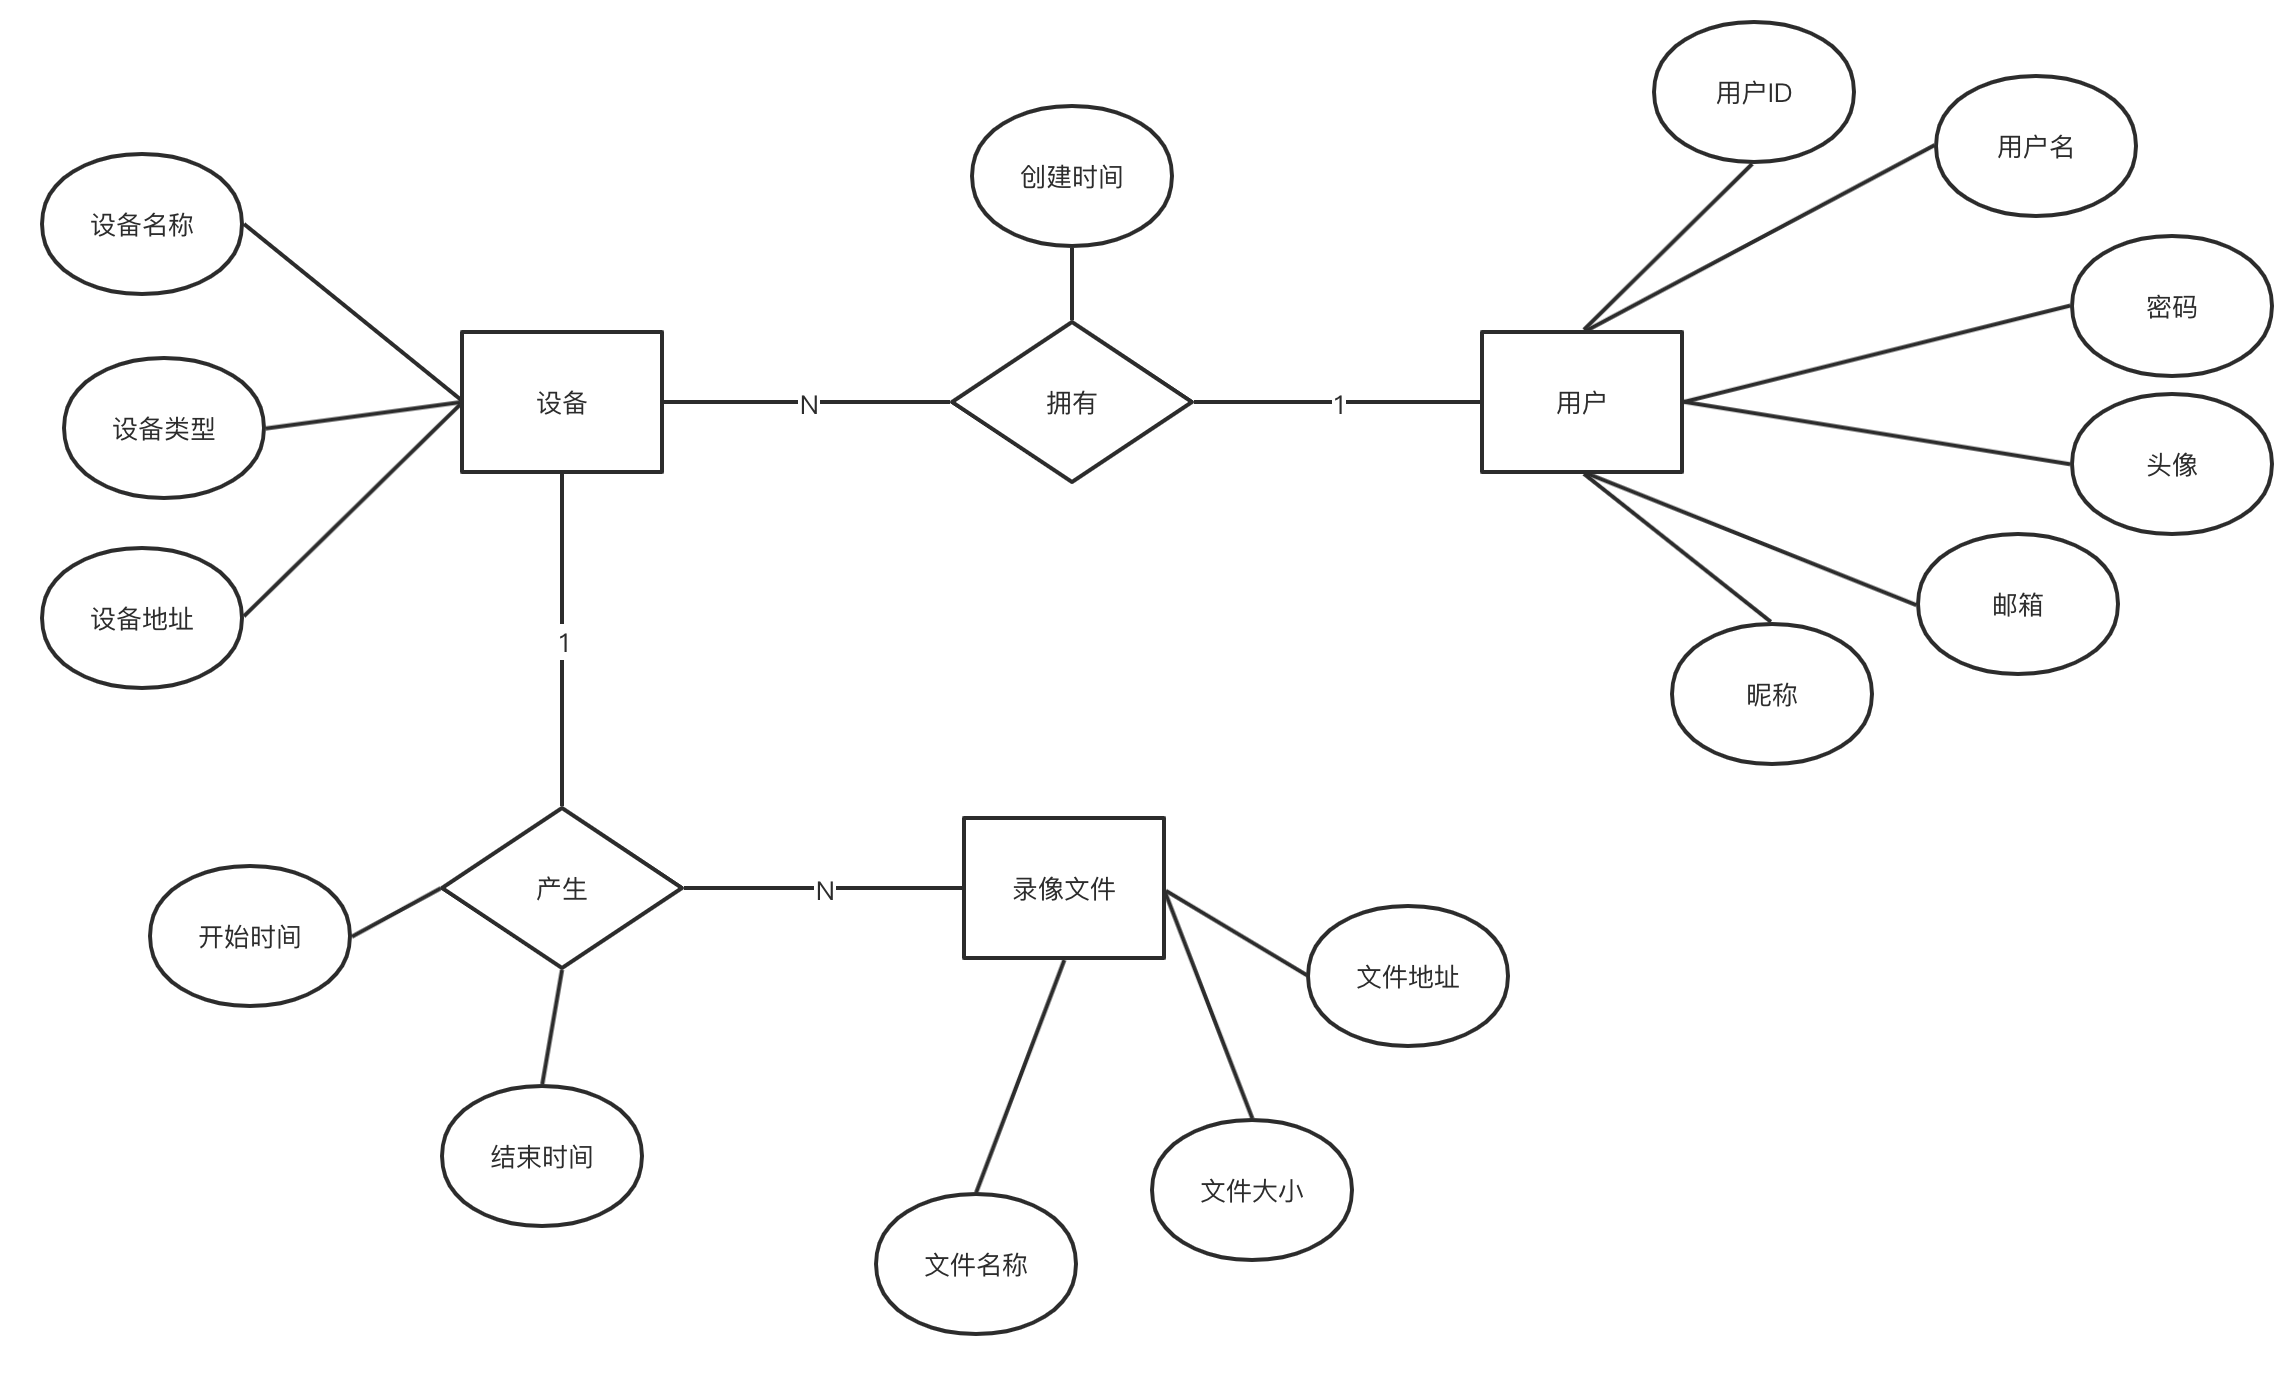
\includegraphics[width=0.5\linewidth]{./Figure/IMG_erd.png}
    \caption{实体关系图}\label{Fig:erd}
\end{figure}

通过实体关系图,可以推导出数据库表结构和表关系,同样如下图所示。

\begin{figure}[ht]
    \centering
    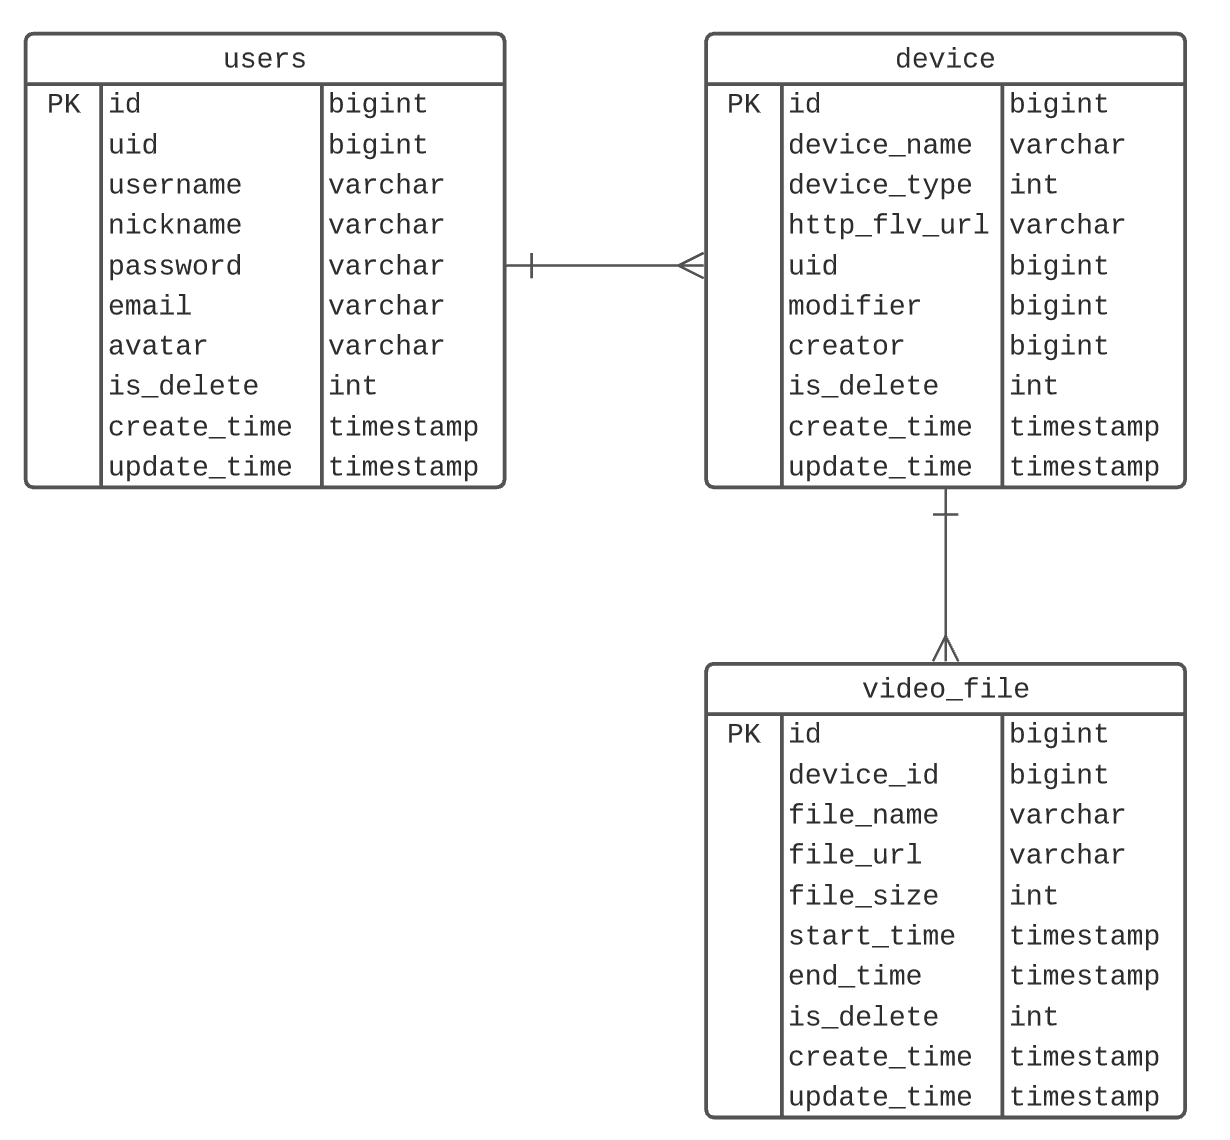
\includegraphics[width=0.5\linewidth]{./Figure/IMG_db.png}
    \caption{数据库表结构和表关系}\label{Fig:db}
\end{figure}

\section{交互接口设计}

\section{系统模块设计}
系统设计分为五个模块,如下表所示


\begin{longtable}[c]{C{5cm}C{7cm}}
    \caption{这是一个长表格}\label{Tab:longtable}\\
    \hline
    模块名称 & 模块功能\\
    % \hline
    % monitoring-system-common&提供公共工具的能力\\ %公共模块
    % \hline
    % monitoring-system-repo&提供数据存储的能力\\ %数据存储模块
    % \hline
    % monitoring-system-service&系统的主要业务逻辑\\ % 业务逻辑模块
    % \hline
    % monitoring-system-media&离线视频文件的存取\\ % 视频文件存取模块
    % \hline
    % monitoring-system-web&为前端提供接口交互\\ %前端接口交互模块
    % \hline

    \hline
    公共模块&提供公共工具的能力\\ %
    \hline
    数据存储模块&提供持久组件的读写的能力\\ %
    \hline
    业务逻辑模块&系统的主要业务逻辑\\ % 
    \hline
    视频文件存取模块&离线视频文件的存取\\ % 
    \hline
    前端接口交互模块&为前端提供接口交互\\ %
    \hline
\end{longtable}
\subsection{公共模块}
公共模块(monitoring-system-common)提供公共工具的能力。
模块内主要包括开发过程中需要用到的注解(annotation)、常量(constant)、枚举(enumerate)、
异常(exception)以及公共的工具封装(utility)。

公共模块中封装的工具包括时间转换工具类、HTTP请求工具类、Spring工具类以及登陆验证码工具类。

时间转换工具类提供将java.util.Date对象转为具有一定格式的字符串(例如“yyyy-MM-dd HH:mm:ss”),
同时也提供逆向转换的能力,即将字符串格式的时间转化为java.util.Date对象。
% 为什么需要

HTTP请求工具类封装了HTTP请求中相关的GET、POST两种请求方法,借助第三方依赖OkHttp二次开发实现。
支持带参数的GET请求、带请求体参数的POST请求。

Spring工具类提供了对Spring上下文的ApplicationContext的静态访问,
可以在全局状态下任何一个地方访问上下文,即可以访问容器内管理的对象和使用Spring提供的观察者模式。

登陆验证码工具类主要提供在登录时生产验证码图片,如下图所示。

\begin{figure}[ht]
    \centering
    
\includegraphics[width=0.5\linewidth]{./Figure/IMG_code.png}
    \caption{登陆验证码}\label{Fig:code}
\end{figure}

\subsection{数据存储模块}
数据存储模块(monitoring-system-repo)提供持久组件的读写的能力。持久组件就是提供数据存储的服务,
在本系统的设计中,持久组件包括MySQL数据库、Reids内存数据库、本地文件系统。

系统设计使用 Mybatis 框架对数据库进行访问,因此该模块中的大部分代码有时有 Mybatis-Generator
自动生成,包括实体对象类、Mapper接口和Mapper配置文件。除此之外,该模块还包括了各种实体的封装类,
比如前端参数封装类(用于封装前端传递给后端的参数)、HTTP响应类(封装后端接口返回对象)
以及各个模块使用的实体类(VO、BO)。

该模块还负责对象之间的转换,即将VO转换成BO或者将BO转换成BO等。该功能是通过对象拷贝技术MapStruct生成的对象转换代码实现的。

\subsection{业务逻辑模块}
业务逻辑模块(monitoring-system-service)提供业务逻辑处理的功能。
该模块是本系统最核心的一个模块,主要负责业务模块的逻辑应用设计,支持登陆鉴权、设备信息的增删改查、个人信息修改等。

业务逻辑模块的主要设计思路是面向接口编程。
接口主要用于描述类具有什么功能,而并不给出每个功能的具体实现。
一个类可以实现一个或多个接口,并在需要接口的地方,随时使用实现了相应接口的对象。

首先设计接口,再设计其对应的实现的类,接着利用Spring的依赖注入特性,
就可以在上层模块声明接口类型的变量,而无需关心其具体实现。
换句话说,业务逻辑模块的变动不会对上层模块的调用产生任何影响。

这就是软件六大设计原则之一的依赖倒置原则,即面向接口编程。
上层模块不应该依赖底层模块,它们都应该依赖于抽象。
抽象不应该依赖于细节,细节应该依赖于抽象。
上层模块不应依赖底层模块,即上层的业务模块不应该依赖底层的实现模块。
如:人出行使用交通工具,只需要知道是交通工具就可以,不用知道是哪种具体的交通工具。
抽象不应该依赖于细节,细节应该依赖于抽象。
在具体的Java编程中,抽象指代接口、抽象函数,统称为接口,而细节指代接口的具体实现。

\subsection{视频文件存取模块}
视频文件存取模块(monitoring-system-media)提供实时监控视频录制和离线查看检索功能。
该模块提供了两个HTTP的接口,分别是监控回放文件的列表查询接口和监控回放文件下载接口。
对于已经在本系统中绑定的监控摄像头设备,每隔一分钟视频文件存取模块会执行定时任务,
对该设备进行录制,并且录制的时长为80秒,目的是做到前后视频文件能有重合部分,防止视频数据丢失。

对于视频文件的存放,可以在本地文件系统和云存储之间无缝切换。
云存储采用阿里云的OSS对象存储服务或本地搭建的Hadoop分布式存储系统。
对于视频文件的读取,该模块提供了一个GET 方法的HTTP接口,入参为视频文件的名称,返回值为该文件内容。
同时还提供搜索功能,支持按照监控视频的开始时间和结束时间进行范围查找。


\subsection{前端接口交互模块}
前端接口交互模块(monitoring-system-web)提供与前端交互的能力。
该模块负责接受前端的请求,然后调用下层模块(如视频文件存取模块)提供的接口方法,实现业务逻辑,
然后将下层模块的返回值进行一定程度的封装后返回给前端进行展示。





\section{权限系统设计}



























\chapter{系统实现}
